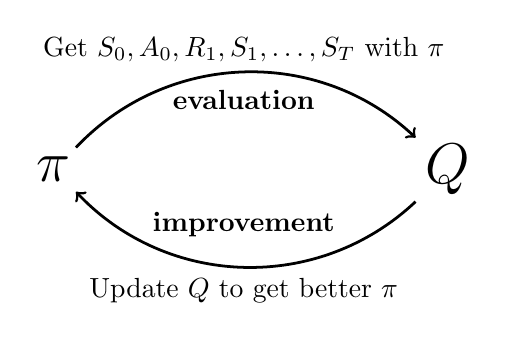
\begin{tikzpicture}
	
	% Create nodes
	\node (A) {\huge$\pi$};
	\node[right of=A, node distance=5cm] (B) {\huge$Q$};
	
	% Create arrow
	\draw[->, line width=1pt] (A) edge[bend left=45] node[below=0.1cm] {\textbf{evaluation}} node[above] {Get $S_0, A_0, R_1, S_1,\dots,S_T$ with $\pi$} (B);
	
	% Create arrow
	\draw[->, line width=1pt] (B) edge[bend left=45] node[below] {Update $Q$ to get better $\pi$} node[above=0.25cm] {\textbf{improvement}} (A);
	
\end{tikzpicture}